%!TEX root = ../../thesis.tex

Background modelling is of paramount importance to the \HWW search. As an irreducible 
background, continuum \WWlvlv production dominates the 0-jet and 1-jet bins, where the 
majority of the sensitivity lies. Thus, even a small uncertainty in this background can 
have a large effect in the fitting procedure. The process is also of general interest to 
electroweak physics and is sensitive to anomalous triple gauge couplings (aTGCs), as seen 
in \Figure~\ref{fig:WW:feyn}.

\begin{figure}[b]
	\null\hfill
	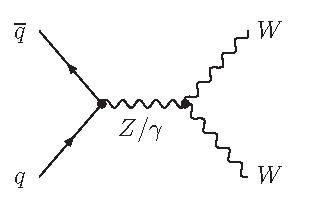
\includegraphics[height=3cm]{axodraw/WW_schannel.pdf}
	\hfill
	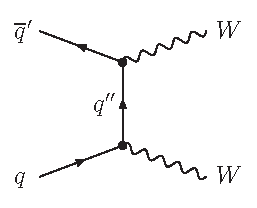
\includegraphics[height=3cm]{axodraw/WW_tchannel.pdf}
	\hfill\null
	\caption{LO Feynman diagrams for \WW production, for the $s$-channel (left) and 
	$t$-channel (right). The $s$-channel contains a triple gauge coupling vertex.}
	\label{fig:WW:feyn}
\end{figure}

\Section~\ref{sec:ww_meas} describes a dedicated \WW cross section measurement performed 
using the 2011 dataset of \pp collisions at \unit{$\sqrt{s} = 7$}{\TeV}. Then, 
\Section~\ref{sec:ww_as_bkg} describes how the \WW background is estimated in the phase 
space of the \HWW search.

